% paper/part1_main.tex
% Part 1: HoloForge — Systematic Degradation Analysis in Phase-Only Computational Holography
% Target: arXiv preprint (cs.GR / eess.IV / physics.optics). Intended as a
%          reproducible simulation study suitable for a workshop / short paper
%          (e.g. SID Display Week, OPTICA Digital Holography) -- NOT framed as a
%          full journal article.
%
% Build:  pdflatex part1_main.tex  (x2 for references)
%         Figures are resolved via \graphicspath (see preamble): drop the PNGs
%         from holography_sandbox/results/ into ./figures/ for submission, or
%         build in place against ../holography_sandbox/results/.
%
% NOTE ON NUMBERS: every quantitative value in this draft is taken verbatim from
% the experiment outputs in ../holography_sandbox/results/ produced by
% run_experiments.py (commit-tracked CSVs: metrics_summary.csv,
% multi_scene_summary.csv, seed_sensitivity_summary.csv). Single-scene values
% refer to the gaussian_spots reference scene; "across scenes" values are the
% mean +/- std over the five-scene suite.

\documentclass[conference]{IEEEtran}
\usepackage{amsmath,amssymb,graphicx,booktabs,hyperref,cite,xcolor}
\usepackage[utf8]{inputenc}
\usepackage[T1]{fontenc}
% Figures: search a local ./figures/ dir first (for submission), then the
% in-repo results directory (for building against freshly generated outputs).
\graphicspath{{figures/}{../holography_sandbox/results/}}

% ─── Metadata ────────────────────────────────────────────────────────────────
\title{Systematic Degradation Analysis in Phase-Only\\Computational Holography: A Simulation Framework}

\author{
  \IEEEauthorblockN{[Author One]}
  \IEEEauthorblockA{[Institution]\\
  [City, Country]\\
  [author.one@institution.edu]}
  \and
  \IEEEauthorblockN{[Author Two]}
  \IEEEauthorblockA{[Institution]\\
  [City, Country]\\
  [author.two@institution.edu]}
  \and
  \IEEEauthorblockN{[Author Three]}
  \IEEEauthorblockA{[Institution]\\
  [City, Country]\\
  [author.three@institution.edu]}
}

\begin{document}
\maketitle

% ─── Abstract ────────────────────────────────────────────────────────────────
\begin{abstract}
Phase-only spatial light modulators (SLMs) are the dominant hardware substrate
for real-time holographic display, but the practical trade-offs between SLM
hardware constraints and reconstruction quality remain incompletely characterised
in a systematic, reproducible way. We present \textsc{HoloForge}, an open-source
Python simulation framework that isolates four independently controllable
degradation axes---spatial resolution, phase quantisation bit-depth,
viewing-angle bandwidth, and coherent speckle noise---and measures their impact
on holographic reconstruction quality using three complementary metrics: PSNR,
SSIM, and LPIPS. All degradations are applied in the physically correct domain:
resolution and bandwidth limits act on the complex SLM field, and speckle is
modelled as random aperture-plane phase noise prior to coherent propagation
rather than as additive intensity noise. Across parameter sweeps on five
test scenes (four synthetic plus one natural photograph) and five random
phase-retrieval seeds, we find phase quantisation to be perceptually lossless
down to 4 bits and near-lossless at 2 bits ($\text{SSIM} = 0.98$ on the
reference scene), with a systematic, theoretically predicted fidelity penalty at
1 bit ($\text{SSIM} = 0.66$ on the reference scene; $0.27 \pm 0.20$ across
scenes, the low end driven by high-frequency content such as the natural
photograph and resolution chart) attributable to the unavoidable twin image of a
real-valued binary phase hologram. We further observe
near-lossless reconstruction of low-spatial-frequency content down to $25\%$
viewing-angle bandwidth ($\text{SSIM} > 0.97$), and a systematic divergence
between PSNR and SSIM under resolution loss, where PSNR stays moderate while
SSIM registers structural collapse. The framework, experiment scripts, and raw result
data are released at \url{https://github.com/ultramagnus23/HoloForge} as a
reproducible baseline for Part~2, which will establish perceptual detection
thresholds via a human-observer study.
\end{abstract}

\begin{IEEEkeywords}
holography, spatial light modulator, phase retrieval, Gerchberg--Saxton,
angular spectrum method, image quality metrics, SSIM, LPIPS, degradation analysis
\end{IEEEkeywords}

% ─── 1. Introduction ─────────────────────────────────────────────────────────
\section{Introduction}
Holographic near-eye displays have attracted sustained research attention as a
candidate for true-depth augmented and virtual reality~\cite{maimone2017holographic,
shi2021towards}. Phase-only SLMs offer the computational tractability of
Fourier-domain phase holography while satisfying the energy-conservation
constraint required for optical efficiency. In practice, however, holographic
reconstruction quality is constrained by several hardware and optical factors:
the spatial resolution of the SLM pixel array, the number of addressable phase
levels (bit-depth), the angular bandwidth subtended by the display aperture
(which determines the usable field of view), and coherent noise introduced by
SLM surface roughness and laser speckle.

These factors have been studied extensively, but almost always \emph{in the
course of proposing a new method}: phase quantisation and fast, heavily-quantised
SLMs in the context of time-multiplexed neural holography~\cite{choi2022time};
speckle and image fidelity in camera-in-the-loop and gradient-based
CGH~\cite{peng2020neural, chakravarthula2019wirtinger, shi2021towards}; and
viewing angle / field of view through the space--bandwidth product and the
hardware that extends it. What is comparatively rare is a \emph{controlled,
method-agnostic} study that isolates each degradation axis
independently---holding the scene, propagation model, and retrieval algorithm
fixed---with reproducible open code and standardised perceptual metrics. We do
not claim these effects are unknown; rather, we provide a reproducible baseline
that disentangles them, which we have not found assembled in one place.

This paper makes the following contributions:
\begin{enumerate}
  \item We present \textsc{HoloForge}, a Python simulation framework implementing
        the Angular Spectrum Method (ASM) and Gerchberg--Saxton (GS) phase
        retrieval, with four independently controllable degradation axes applied
        in their physically correct domains.
  \item We characterise the bit-depth dependence of GS-computed phase holograms
        and show that the transition to a binary (1-bit) hologram incurs a
        systematic, theoretically predicted fidelity penalty from an unavoidable
        twin image, which we verify is stable across five scenes and five
        random seeds.
  \item We demonstrate that PSNR and SSIM diverge in their characterisation of
        holographic degradation, and that a true LPIPS perceptual metric provides
        complementary information not captured by either.
  \item We release all code, experiment scripts, and raw result data as an
        open-source, reproducible baseline for future work.
\end{enumerate}

The remainder of this paper is organised as follows. Section~\ref{sec:related}
reviews related work. Section~\ref{sec:method} describes the optical model and
simulation framework. Section~\ref{sec:experiments} presents the experimental
protocol. Section~\ref{sec:results} reports results across four degradation axes.
Section~\ref{sec:discussion} interprets the findings and acknowledges
limitations. Section~\ref{sec:conclusion} concludes and outlines Part~2.

% ─── 2. Related Work ─────────────────────────────────────────────────────────
\section{Related Work}
\label{sec:related}

\subsection{Holographic Display Hardware}
Modern holographic displays are built around liquid-crystal-on-silicon (LCoS)
phase-only SLMs, whose key specifications---pixel pitch, panel resolution, and
the number of addressable phase levels---directly bound the achievable space-
bandwidth product and field of view~\cite{holoeye2023slm}. The diffraction
angle of an SLM is set by its pixel pitch ($\sin\theta \approx
\lambda/2\Delta x$), so smaller pixels widen the viewing zone but increase
fabrication cost. The product of field of view and eyebox---the {\'e}tendue---is proportional to
the SLM pixel count, imposing a fundamental trade-off that has motivated
space--bandwidth-product extension and learned {\'e}tendue-expansion hardware.
Pixel count and addressable phase levels are also costly, which has driven
interest in \emph{fast, heavily-quantised} panels: time-multiplexed neural
holography, for instance, explicitly targets low-bit-depth SLMs and compensates
algorithmically~\cite{choi2022time}. Historically, binary (1-bit)
computer-generated holograms were studied extensively because early devices could
not address continuous phase~\cite{brown1966complex,lee1978computer}; the move to
multi-level phase-only SLMs largely supplanted them for display because binary
encodings incur an unavoidable conjugate (twin) image~\cite{gabor1948new}. Our
quantisation sweep revisits this transition quantitatively, in a controlled
setting, under a fixed modern phase-retrieval pipeline.

\subsection{Phase Retrieval}
The Gerchberg--Saxton algorithm~\cite{gerchberg1972practical} alternates
amplitude constraints between the hologram and image planes and remains a
standard baseline for phase-only hologram synthesis. Fienup's input--output
variants~\cite{fienup1982phase} improve convergence and stagnation behaviour,
while recent work casts hologram synthesis as differentiable optimisation
(Wirtinger / gradient-descent holography~\cite{chakravarthula2019wirtinger}) or
learns the encoding directly with neural
networks~\cite{shi2021towards, peng2020neural}. GS is known to converge to lower
reconstruction quality than these gradient-based and camera-in-the-loop methods,
which better suppress speckle and model artefacts~\cite{peng2020neural}. We
nevertheless adopt classical GS precisely \emph{because} it is transparent,
deterministic given a seed, and widely understood---properties that make it a
clean substrate for isolating degradation effects. Characterising the degradation
sensitivity of optimisation-based and neural methods, which may shift the
quantisation and bandwidth thresholds reported here, is left to future work.

\subsection{Image Quality Metrics for Holography}
Peak signal-to-noise ratio (PSNR) measures pixel-level fidelity but is known to
correlate poorly with perceived quality, particularly for structured or
coherent-noise artefacts. The structural similarity index
(SSIM)~\cite{wang2004image} incorporates luminance, contrast, and local structure
and is widely used in display evaluation. Learned perceptual image patch
similarity (LPIPS)~\cite{zhang2018unreasonable} compares deep-network feature
activations and tracks human judgements of perceptual distance more closely than
either PSNR or SSIM on many distortion types. We report all three to expose where
they agree and, importantly, where they diverge under holographic degradation.

% ─── 3. Optical Model and Simulation Framework ───────────────────────────────
\section{Optical Model and Simulation Framework}
\label{sec:method}

\subsection{Angular Spectrum Method}
We model free-space wave propagation using the Angular Spectrum Method
(ASM)~\cite{goodman2005introduction}. For a monochromatic field $U(x,y,0)$ at the
SLM plane, the field at propagation distance $z$ is
\begin{equation}
  U(x,y,z) = \mathcal{F}^{-1}\!\left\{
    \hat{U}(f_x, f_y)\, H(f_x, f_y, z)
  \right\},
\end{equation}
where $\hat{U} = \mathcal{F}\{U\}$ is the angular spectrum and the transfer
function is
\begin{equation}
  H(f_x,f_y,z) =
  \begin{cases}
    \exp\!\left(j 2\pi z \sqrt{\lambda^{-2} - f_x^2 - f_y^2}\right) & f_x^2+f_y^2 \le \lambda^{-2}\\
    0 & \text{(evanescent),}
  \end{cases}
\end{equation}
with wavelength $\lambda = 532\,\text{nm}$, propagation distance
$z = 150\,\text{mm}$, and SLM pixel pitch $\Delta x = 8\,\mu\text{m}$. The
implementation conserves energy to within $1\%$ and is exactly invertible
($U_{-z} \circ U_{z} = \mathrm{Id}$ to numerical precision); both invariants are
asserted in the unit-test suite (Section~\ref{sec:experiments}).

\subsection{Gerchberg--Saxton Phase Retrieval}
We compute phase-only holograms using the Gerchberg--Saxton (GS)
algorithm~\cite{gerchberg1972practical}. Starting from a random initial phase at
the SLM plane, the algorithm alternately enforces the target amplitude constraint
at the image plane and the phase-only constraint at the SLM plane:
\begin{align}
  \text{SLM} &\xrightarrow{\text{ASM}(+z)} \text{Image plane} \\
  &\xrightarrow{\text{amplitude replace}} A_{\text{target}}\, e^{j\angle U_{\text{img}}} \\
  &\xrightarrow{\text{ASM}(-z)} \text{SLM plane} \\
  &\xrightarrow{\text{phase-only}} e^{j\angle U_{\text{SLM}}}.
\end{align}
We run $50$ iterations at resolution $256\times256$ pixels. Convergence is
confirmed by monitoring per-iteration reconstruction MSE
(Section~\ref{sec:results}): the normalised-amplitude MSE falls from
$8.7\times10^{-2}$ at iteration~1 to $7.5\times10^{-4}$ by iteration~30 and
$7.1\times10^{-4}$ by iteration~50, motivating our choice of 50 iterations over
the more common but under-converged 30.

\subsection{Degradation Model}
We define four independently controllable degradation axes, each applied to the
computed phase hologram before reconstruction. Critically, every operator acts
in the physically correct domain.

\textbf{(D1) Spatial Resolution.} The SLM phase is downsampled from $N\times N$
to $n\times n$ pixels using nearest-neighbour interpolation \emph{in the complex
phasor domain} (operating on the real and imaginary parts of $e^{j\phi}$ rather
than on $\phi$ directly, avoiding phase-wrap and $8$-bit quantisation artefacts),
then upsampled back to $N\times N$. We sweep $n \in \{128, 64, 32, 16\}$ against a
baseline of $N=256$.

\textbf{(D2) Phase Quantisation.} The continuous phase is quantised to $2^b$
evenly spaced levels, $b \in \{1, 2, 4, 8\}$ bits, using a mid-rise quantiser
over the periodic phase circle,
\begin{equation}
  \phi_q = \frac{2\pi}{2^b}\!\left(\left\lfloor \frac{(\phi+\pi)\, 2^b}{2\pi} \right\rfloor + \tfrac{1}{2}\right) - \pi.
\end{equation}
The mid-rise form places exactly $2^b$ distinct phasors over $[-\pi,\pi)$; a
na\"ive closed-interval mapping would instead collide $-\pi$ and $+\pi$ (which
share the phasor $-1$) and, at $b=1$, collapse to a single-valued constant
hologram. At $b=1$ the two levels lie $\pi$ apart, yielding a genuine binary
phase hologram.

\textbf{(D3) Viewing-Angle Bandwidth.} The SLM phase is converted to a complex
phasor, its spatial-frequency spectrum is masked to a circular aperture of radius
$\beta \cdot f_{\max}$ (with $f_{\max} = 1/(2\Delta x)$ the Nyquist limit), and
the phase is recovered from the masked field. We sweep
$\beta \in \{1.0, 0.75, 0.5, 0.25, 0.1\}$.

\textbf{(D4) Coherent Speckle.} Random phase perturbations $\delta\phi \sim
\mathcal{N}(0, \sigma^2)$ are added to the SLM phase \emph{before}
reconstruction, modelling surface roughness and SLM phase error. Speckle thus
arises through coherent interference during propagation, reproducing the correct
physical mechanism rather than additive intensity noise. We sweep
$\sigma \in \{0.1, 0.3, 0.6, 1.0, \pi\}$ radians.

Multi-wavelength (RGB) colour holography is explicitly out of scope for Part~1
and is deferred to Part~2. A na\"ive ``colour'' axis that post-processes a
monochrome reconstruction would not model any holographic colour physics, so it
is excluded rather than reported (see the released
\texttt{sweep\_color\_EXCLUDED.txt}). Depth-plane multi-focus holography---in
which several object planes are encoded by coherent superposition of
per-plane holograms---is likewise treated separately and deferred to Part~2; the
released code includes a physically correct complex-field superposition routine
(summing $e^{j\phi}$ across planes rather than the phases themselves) as a
demonstration, but a controlled depth-degradation study requires a depth-aware
reference and metric that are beyond Part~1's single-plane scope.

\subsection{Metrics}
We evaluate reconstruction quality using three complementary metrics:
\begin{itemize}
  \item \textbf{PSNR}---peak signal-to-noise ratio in dB.
  \item \textbf{SSIM}---structural similarity index~\cite{wang2004image}.
  \item \textbf{LPIPS}---learned perceptual image patch similarity
        (AlexNet backbone)~\cite{zhang2018unreasonable}, the true learned metric
        rather than a hand-crafted proxy.
\end{itemize}
PSNR is pixel-level; SSIM accounts for luminance, contrast, and structure; LPIPS
captures perceptual similarity via deep features. Measuring all three allows us to
characterise divergence between physical and perceptual quality estimates---a
central observation in the results.

% ─── 4. Experimental Protocol ────────────────────────────────────────────────
\section{Experimental Protocol}
\label{sec:experiments}

\subsection{Test Scenes}
We evaluate on five scenes that span different spatial-frequency profiles: (1)
\textit{gaussian\_spots}---four Gaussian blobs of varying brightness (the
low-frequency reference scene); (2) \textit{resolution\_chart}---bar gratings at
spatial periods from $4$ to $64$ px/cycle; (3) \textit{letters}---the word
``HOLO'' rendered at $256\times256$; (4) \textit{circle\_ring}---a concentric-ring
pattern testing radial symmetry; and (5) \textit{natural\_photo}---the standard
``cameraman'' photograph (bundled with scikit-image, no download required),
providing broadband natural-image statistics as a counterpoint to the four
synthetic patterns.

\subsection{Statistical Methodology}
Single-scene sweeps (Section~\ref{sec:results}, individual tables) use the
\textit{gaussian\_spots} reference scene. Generalisation is assessed by repeating
the resolution, phase-quantisation, and viewing-angle sweeps on all five scenes
and reporting mean~$\pm$~std across scenes (Table~\ref{tab:multiscene}). Stability
to phase-retrieval initialisation is assessed by repeating the two most critical
sweeps (phase quantisation and resolution) across five random GS seeds
$\{42, 7, 123, 999, 17\}$ and reporting mean~$\pm$~std across seeds
(Table~\ref{tab:seed}). All experiments use $256\times256$ resolution and $50$ GS
iterations.

\subsection{Reproducibility}
The framework ships a \texttt{pytest} suite of ten physics-invariant tests
(ASM energy conservation and round-trip invertibility, GS convergence,
reconstruction range, quantisation level counts, complex-field superposition,
physical-speckle range, and metric sanity checks), all of which pass. The full
result set is regenerated end-to-end by a single command,
\texttt{python run\_experiments.py}, in approximately $35\,\text{s}$ on a CPU.

% ─── 5. Results ──────────────────────────────────────────────────────────────
\section{Results}
\label{sec:results}

\subsection{GS Convergence}
\begin{figure}[t]
  \centering
  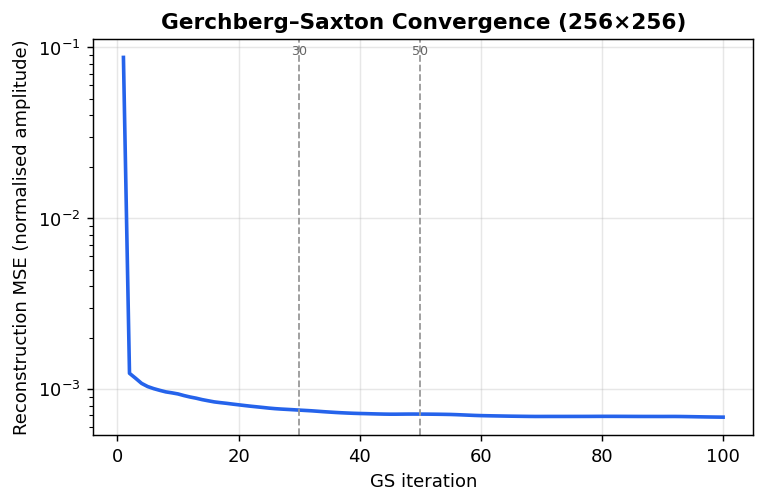
\includegraphics[width=\columnwidth]{gs_convergence.png}
  \caption{GS convergence: per-iteration reconstruction MSE over 100 iterations
  at $256\times256$. The error drops by two orders of magnitude within $\sim$30
  iterations and is essentially flat thereafter; we use 50 iterations throughout.}
  \label{fig:gs_convergence}
\end{figure}
Figure~\ref{fig:gs_convergence} shows the GS reconstruction MSE decreasing from
$8.7\times10^{-2}$ to a plateau near $7\times10^{-4}$. The marginal improvement
from iteration~30 ($7.5\times10^{-4}$) to iteration~50 ($7.1\times10^{-4}$) to
iteration~100 ($6.8\times10^{-4}$) is small, confirming that 50 iterations are
sufficient while 30 leave a modest residual.

\subsection{D1: Spatial Resolution}
\begin{figure}[t]
  \centering
  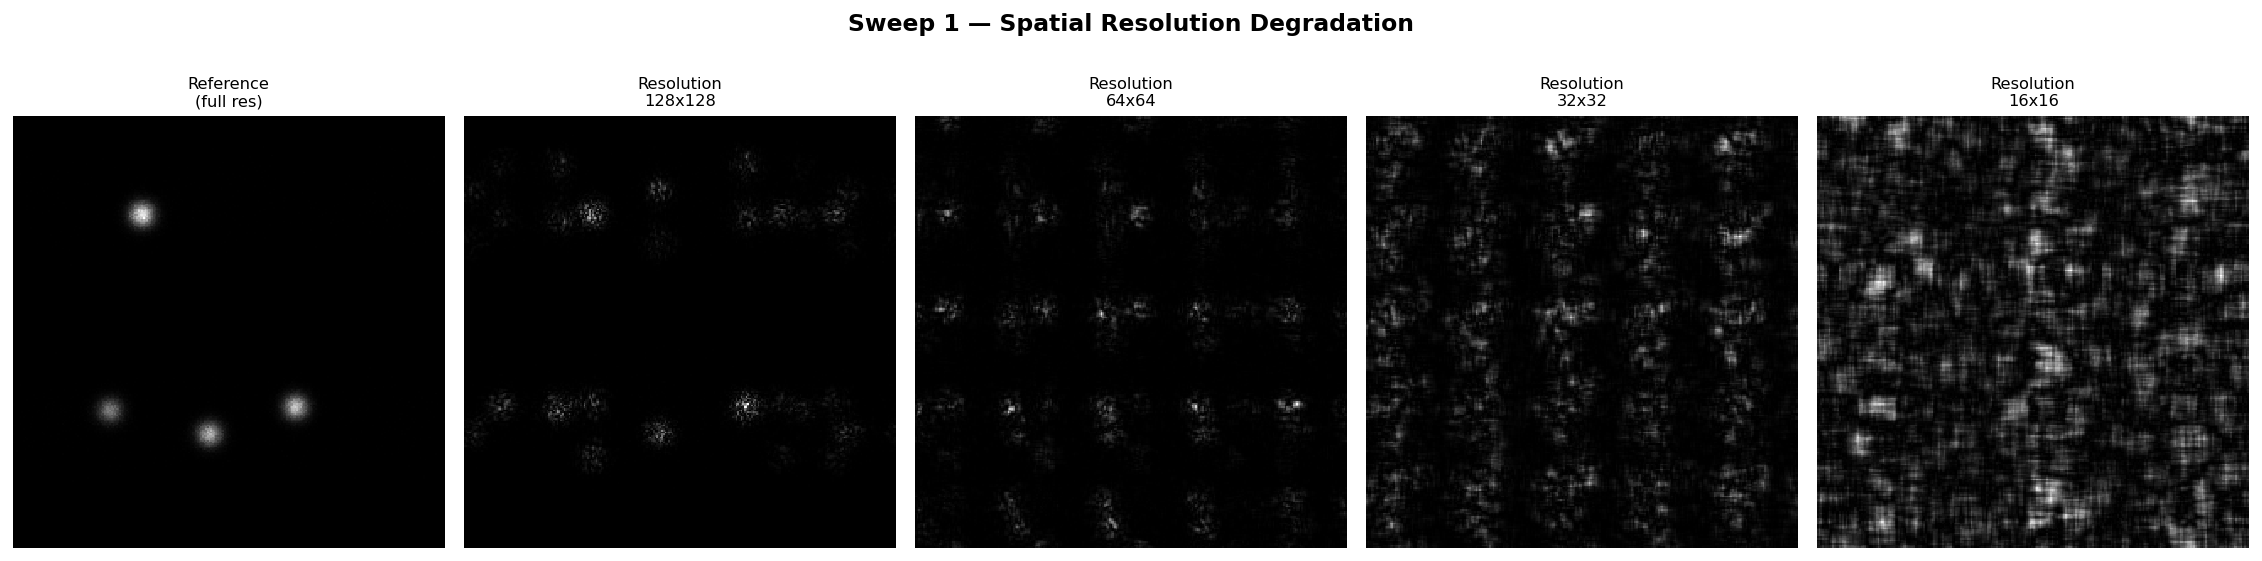
\includegraphics[width=\columnwidth]{sweep_resolution.png}
  \caption{Resolution degradation: reconstructions at effective SLM resolutions
  of $256$, $128$, $64$, $32$, and $16$ pixels (complex-domain downsampling).}
  \label{fig:resolution}
\end{figure}
\begin{table}[t]
  \centering
  \caption{Resolution sweep (mean $\pm$ std across five scenes)}
  \label{tab:resolution}
  \begin{tabular}{lccc}
    \toprule
    Resolution & PSNR (dB) & SSIM & LPIPS \\
    \midrule
    128$\times$128 & $17.03 \pm 6.69$ & $0.388 \pm 0.313$ & $0.659 \pm 0.220$ \\
    64$\times$64   & $15.99 \pm 5.74$ & $0.228 \pm 0.231$ & $0.705 \pm 0.085$ \\
    32$\times$32   & $14.66 \pm 4.03$ & $0.085 \pm 0.072$ & $0.757 \pm 0.045$ \\
    16$\times$16   & $13.05 \pm 2.22$ & $0.052 \pm 0.020$ & $0.837 \pm 0.075$ \\
    \bottomrule
  \end{tabular}
\end{table}
Resolution degradation is monotonic across all three metrics
(Table~\ref{tab:resolution}). The across-scene standard deviations are large
because survival under resolution reduction is governed by the target's
spatial-frequency content relative to the SLM space--bandwidth budget: on the
low-frequency reference scene the decline is graceful ($\text{SSIM} = 0.860$ at
$128\times128$, $0.657$ at $64\times64$), whereas high-frequency content such as
\textit{resolution\_chart} and the fine detail of \textit{natural\_photo}
collapses almost immediately once the effective pixel count can no longer
represent it. The variance is thus not noise but a measurable signature of
content-dependent bandwidth demand.

\subsection{D2: Phase Quantisation}
\begin{figure}[t]
  \centering
  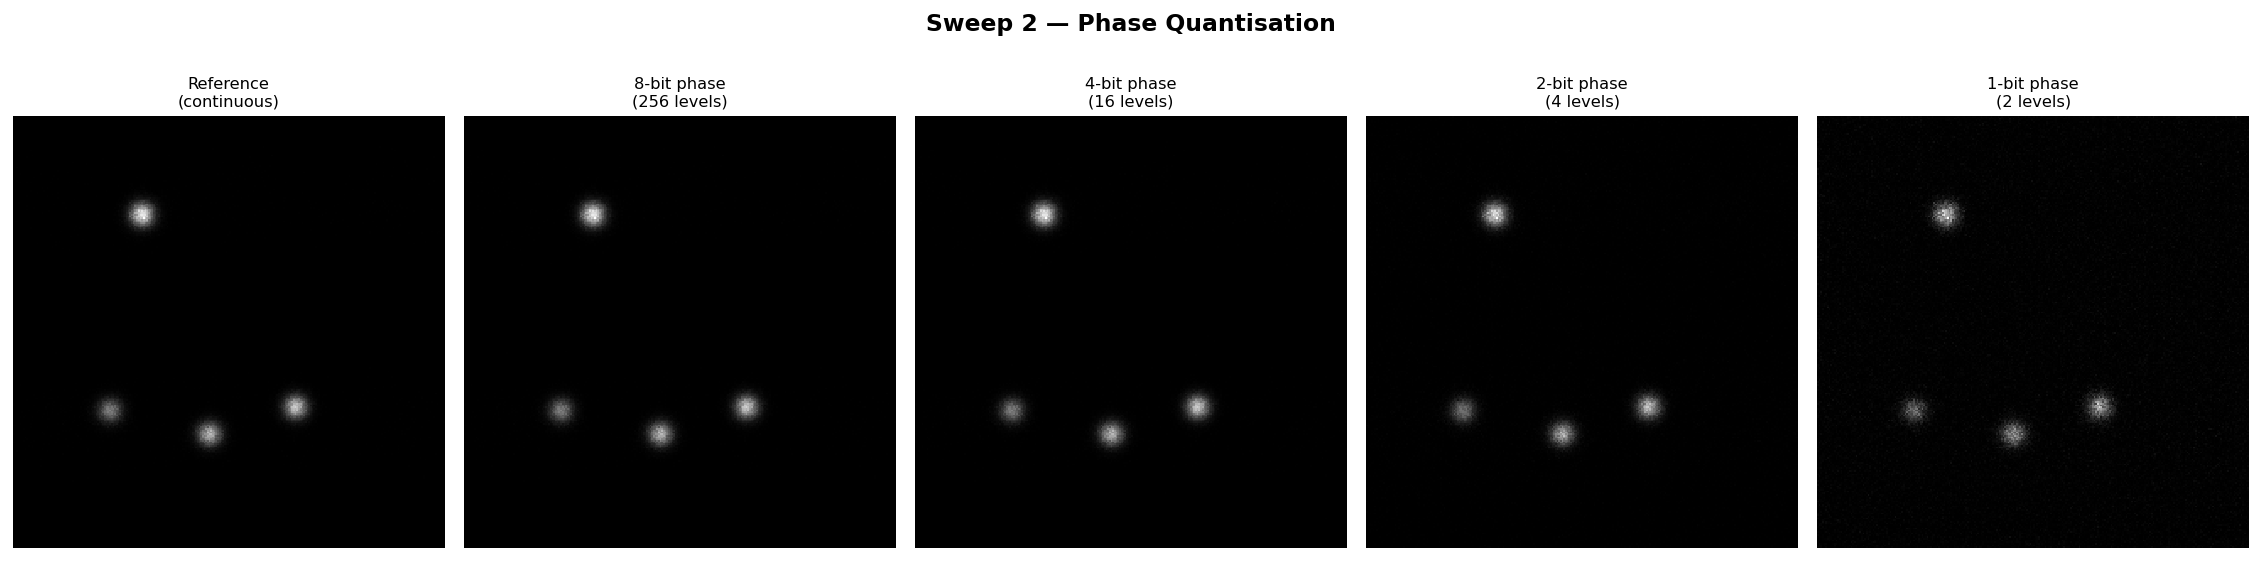
\includegraphics[width=\columnwidth]{sweep_phase_bits.png}
  \caption{Phase quantisation: reconstructions at 8, 4, 2, and 1 bit(s). The
  1-bit (binary phase) case retains coarse structure but loses fidelity to an
  unavoidable twin image.}
  \label{fig:phase_bits}
\end{figure}
\begin{table}[t]
  \centering
  \caption{Phase quantisation sweep (reference scene; across-scene mean in text)}
  \label{tab:phase_bits}
  \begin{tabular}{lccc}
    \toprule
    Phase bits & PSNR (dB) & SSIM & LPIPS \\
    \midrule
    8-bit & $83.0$ & $1.000$ & $0.000$ \\
    4-bit & $59.4$ & $1.000$ & $0.000$ \\
    2-bit & $45.0$ & $0.978$ & $0.016$ \\
    1-bit & $35.7$ & $0.655$ & $0.180$ \\
    \bottomrule
  \end{tabular}
\end{table}
\textbf{Key finding.} Phase quantisation is perceptually lossless down to 4 bits
and near-lossless at 2 bits, with a systematic fidelity penalty at the 1-bit
(binary) transition (Table~\ref{tab:phase_bits}, Fig.~\ref{fig:phase_bits}). On
the reference scene SSIM is $1.000$ at 4 and 8 bits, $0.978$ at 2 bits, and
$0.655$ at 1 bit, while PSNR declines smoothly
($83.0 \to 59.4 \to 45.0 \to 35.7\,\text{dB}$). Across the five scenes the 1-bit
case is more content-sensitive (SSIM $0.273\pm0.198$) but the ordering is
preserved. Crucially, the 1-bit loss is \emph{systematic rather than
stochastic}: across five random GS seeds the 1-bit SSIM is $0.600\pm0.028$
(Table~\ref{tab:seed}), a tight distribution indicating the degradation is
structural, not an artefact of initialisation. Section~\ref{sec:discussion}
identifies this loss as the signature of an unavoidable twin image and predicts
its onset at exactly 1 bit.

\subsection{D3: Viewing-Angle Bandwidth}
\begin{figure}[t]
  \centering
  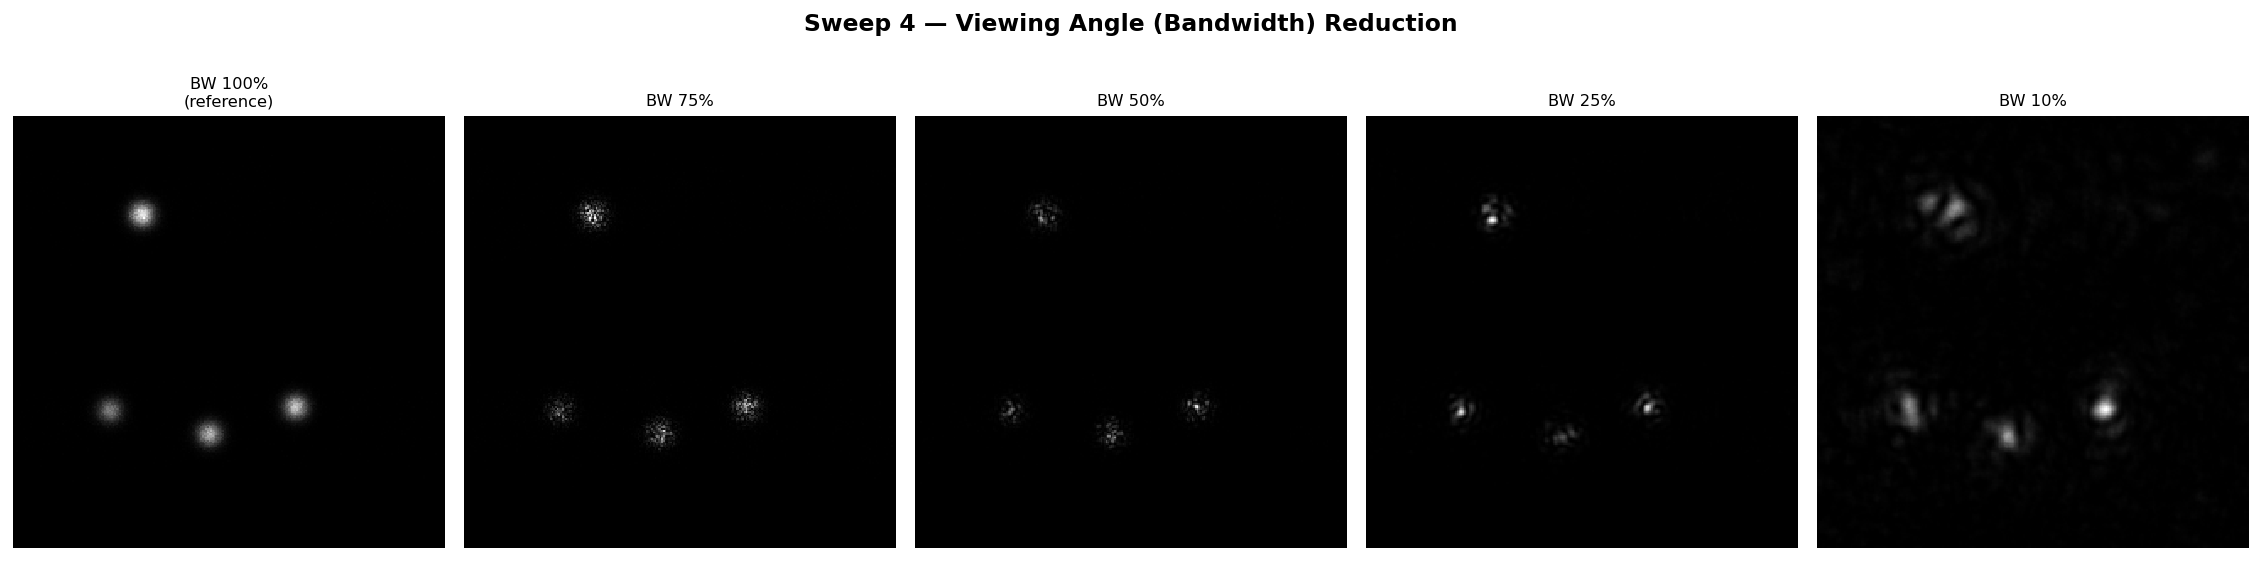
\includegraphics[width=\columnwidth]{sweep_viewing_angle.png}
  \caption{Viewing-angle bandwidth reduction to $75\%$, $50\%$, $25\%$, and
  $10\%$ of the Nyquist limit. Low-frequency content tolerates aggressive
  bandwidth reduction.}
  \label{fig:viewing_angle}
\end{figure}
\begin{table}[t]
  \centering
  \caption{Viewing-angle sweep (mean $\pm$ std across five scenes)}
  \label{tab:viewing}
  \begin{tabular}{lccc}
    \toprule
    Bandwidth & PSNR (dB) & SSIM & LPIPS \\
    \midrule
    75\% & $18.37 \pm 7.28$ & $0.634 \pm 0.293$ & $0.402 \pm 0.232$ \\
    50\% & $17.46 \pm 6.72$ & $0.615 \pm 0.297$ & $0.420 \pm 0.244$ \\
    25\% & $17.47 \pm 7.02$ & $0.595 \pm 0.306$ & $0.435 \pm 0.257$ \\
    10\% & $17.44 \pm 6.66$ & $0.362 \pm 0.202$ & $0.540 \pm 0.221$ \\
    \bottomrule
  \end{tabular}
\end{table}
Viewing-angle reduction is the gentlest of the four axes
(Table~\ref{tab:viewing}). On the low-frequency reference scene SSIM remains
above $0.97$ down to $25\%$ bandwidth and only falls to $0.728$ at $10\%$. Across
all scenes the mean SSIM declines slowly from $0.634$ ($75\%$) to $0.615$
($50\%$) to $0.595$ ($25\%$) before dropping to $0.362$ at $10\%$.

The near-flat $50\%\!\to\!25\%$ region warrants explanation, since one might
suspect the bandwidth mask is inert there. It is not: measuring the fraction of
hologram spectral energy that survives the circular mask shows monotone, large
removal at every step---on average $0.80$, $0.46$, $0.21$, $0.055$, and $0.008$
of the total energy is retained at $100/75/50/25/10\%$ bandwidth. The operator
therefore discards $\sim\!95\%$ of the spectral energy by $25\%$ bandwidth. SSIM
nonetheless plateaus because reconstruction quality is governed not by total
retained energy but by whether the \emph{energy-bearing low-frequency core}
survives: for compact, low-frequency targets that core lies within the $25\%$
disc, so masking between $75\%$ and $25\%$ removes mostly low-energy
high-frequency components to which a phase-only reconstruction is insensitive,
whereas the sharp drop at $10\%$ coincides with the mask finally cutting into the
core (retained energy $0.055\!\to\!0.008$). This is strongly
content-dependent---and the flat average superimposes two distinct behaviours:
low-frequency scenes are flat-then-cliff (\textit{gaussian\_spots}
$0.978\!\to\!0.972$ from $75\%$ to $25\%$, then $0.728$ at $10\%$), whereas
broadband scenes are already largely lost at $75\%$ and decline gradually
(\textit{natural\_photo} $0.237\!\to\!0.218\!\to\!0.163$). The wide across-scene
standard deviation in Table~\ref{tab:viewing} is the signature of this split, not
of operator inactivity.

\subsection{D4: Coherent Speckle}
\begin{figure}[t]
  \centering
  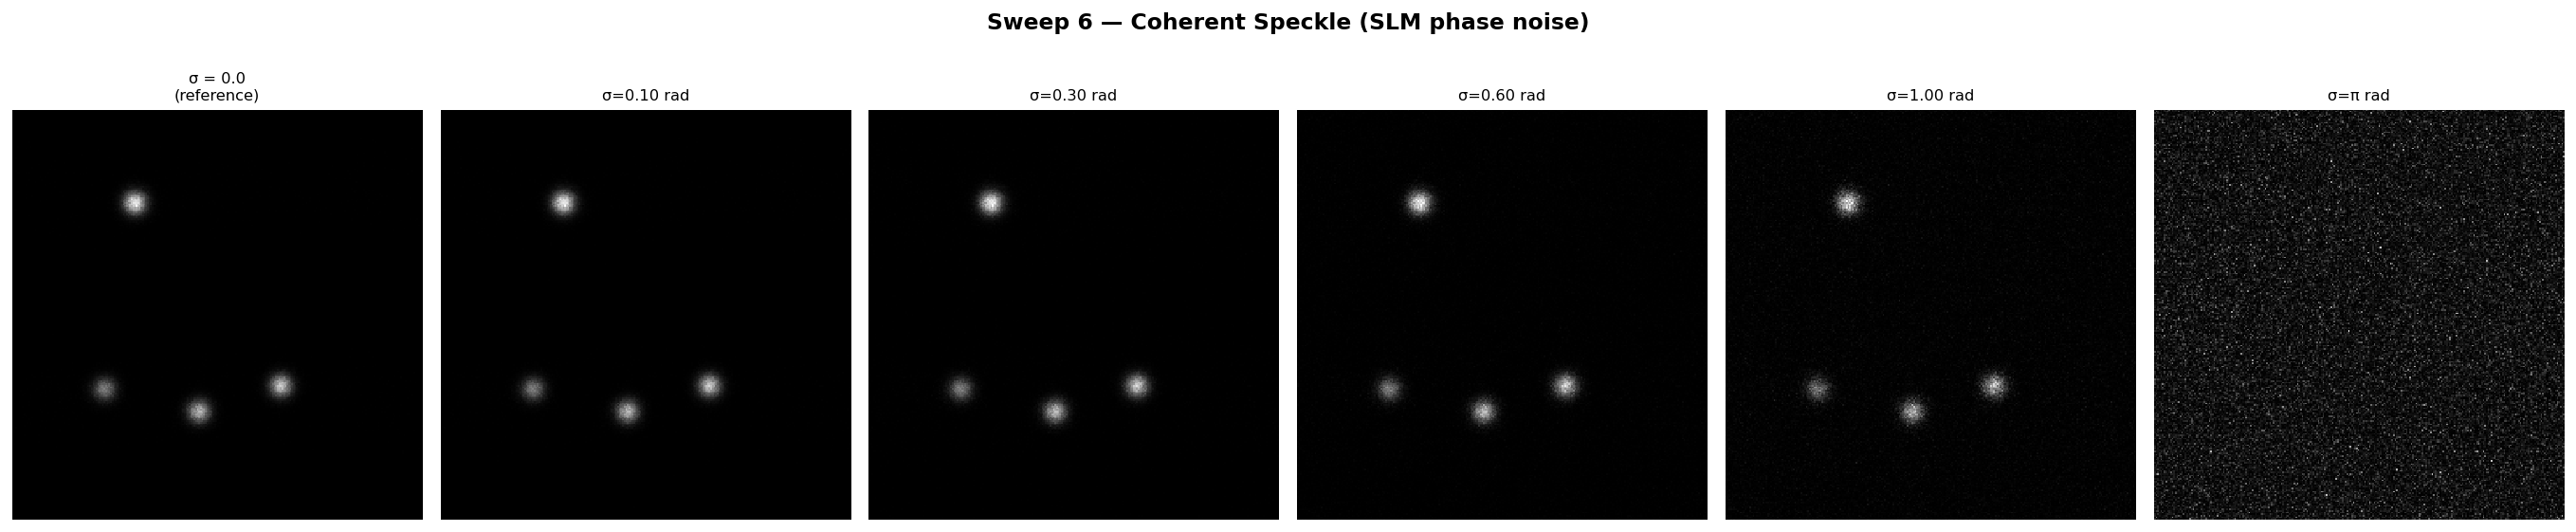
\includegraphics[width=\columnwidth]{sweep_speckle.png}
  \caption{Coherent speckle from aperture-plane phase noise of increasing std
  $\sigma$. Reconstruction remains near-perfect up to $\sigma\approx0.3$ rad and
  collapses as $\sigma\to\pi$.}
  \label{fig:speckle}
\end{figure}
\begin{table}[t]
  \centering
  \caption{Coherent speckle sweep (reference scene)}
  \label{tab:speckle}
  \begin{tabular}{lccc}
    \toprule
    $\sigma$ (rad) & PSNR (dB) & SSIM & LPIPS \\
    \midrule
    0.10 & $60.1$ & $1.000$ & $0.000$ \\
    0.30 & $49.7$ & $0.994$ & $0.005$ \\
    0.60 & $42.7$ & $0.915$ & $0.053$ \\
    1.00 & $34.9$ & $0.501$ & $0.258$ \\
    $\pi$ & $18.5$ & $0.008$ & $0.963$ \\
    \bottomrule
  \end{tabular}
\end{table}
Coherent speckle exhibits a soft knee (Table~\ref{tab:speckle}): the
reconstruction is essentially unaffected for $\sigma \le 0.3\,\text{rad}$
($\text{SSIM} \ge 0.99$), degrades through $\sigma = 0.6$ ($0.915$) and
$\sigma = 1.0$ ($0.501$), and is destroyed as the perturbation approaches a
uniform random phase at $\sigma = \pi$ ($\text{SSIM} = 0.008$). This provides a
quantitative tolerance budget for SLM phase accuracy and optical-surface quality.

\subsection{Metric Divergence and Generalisation}
\begin{figure}[t]
  \centering
  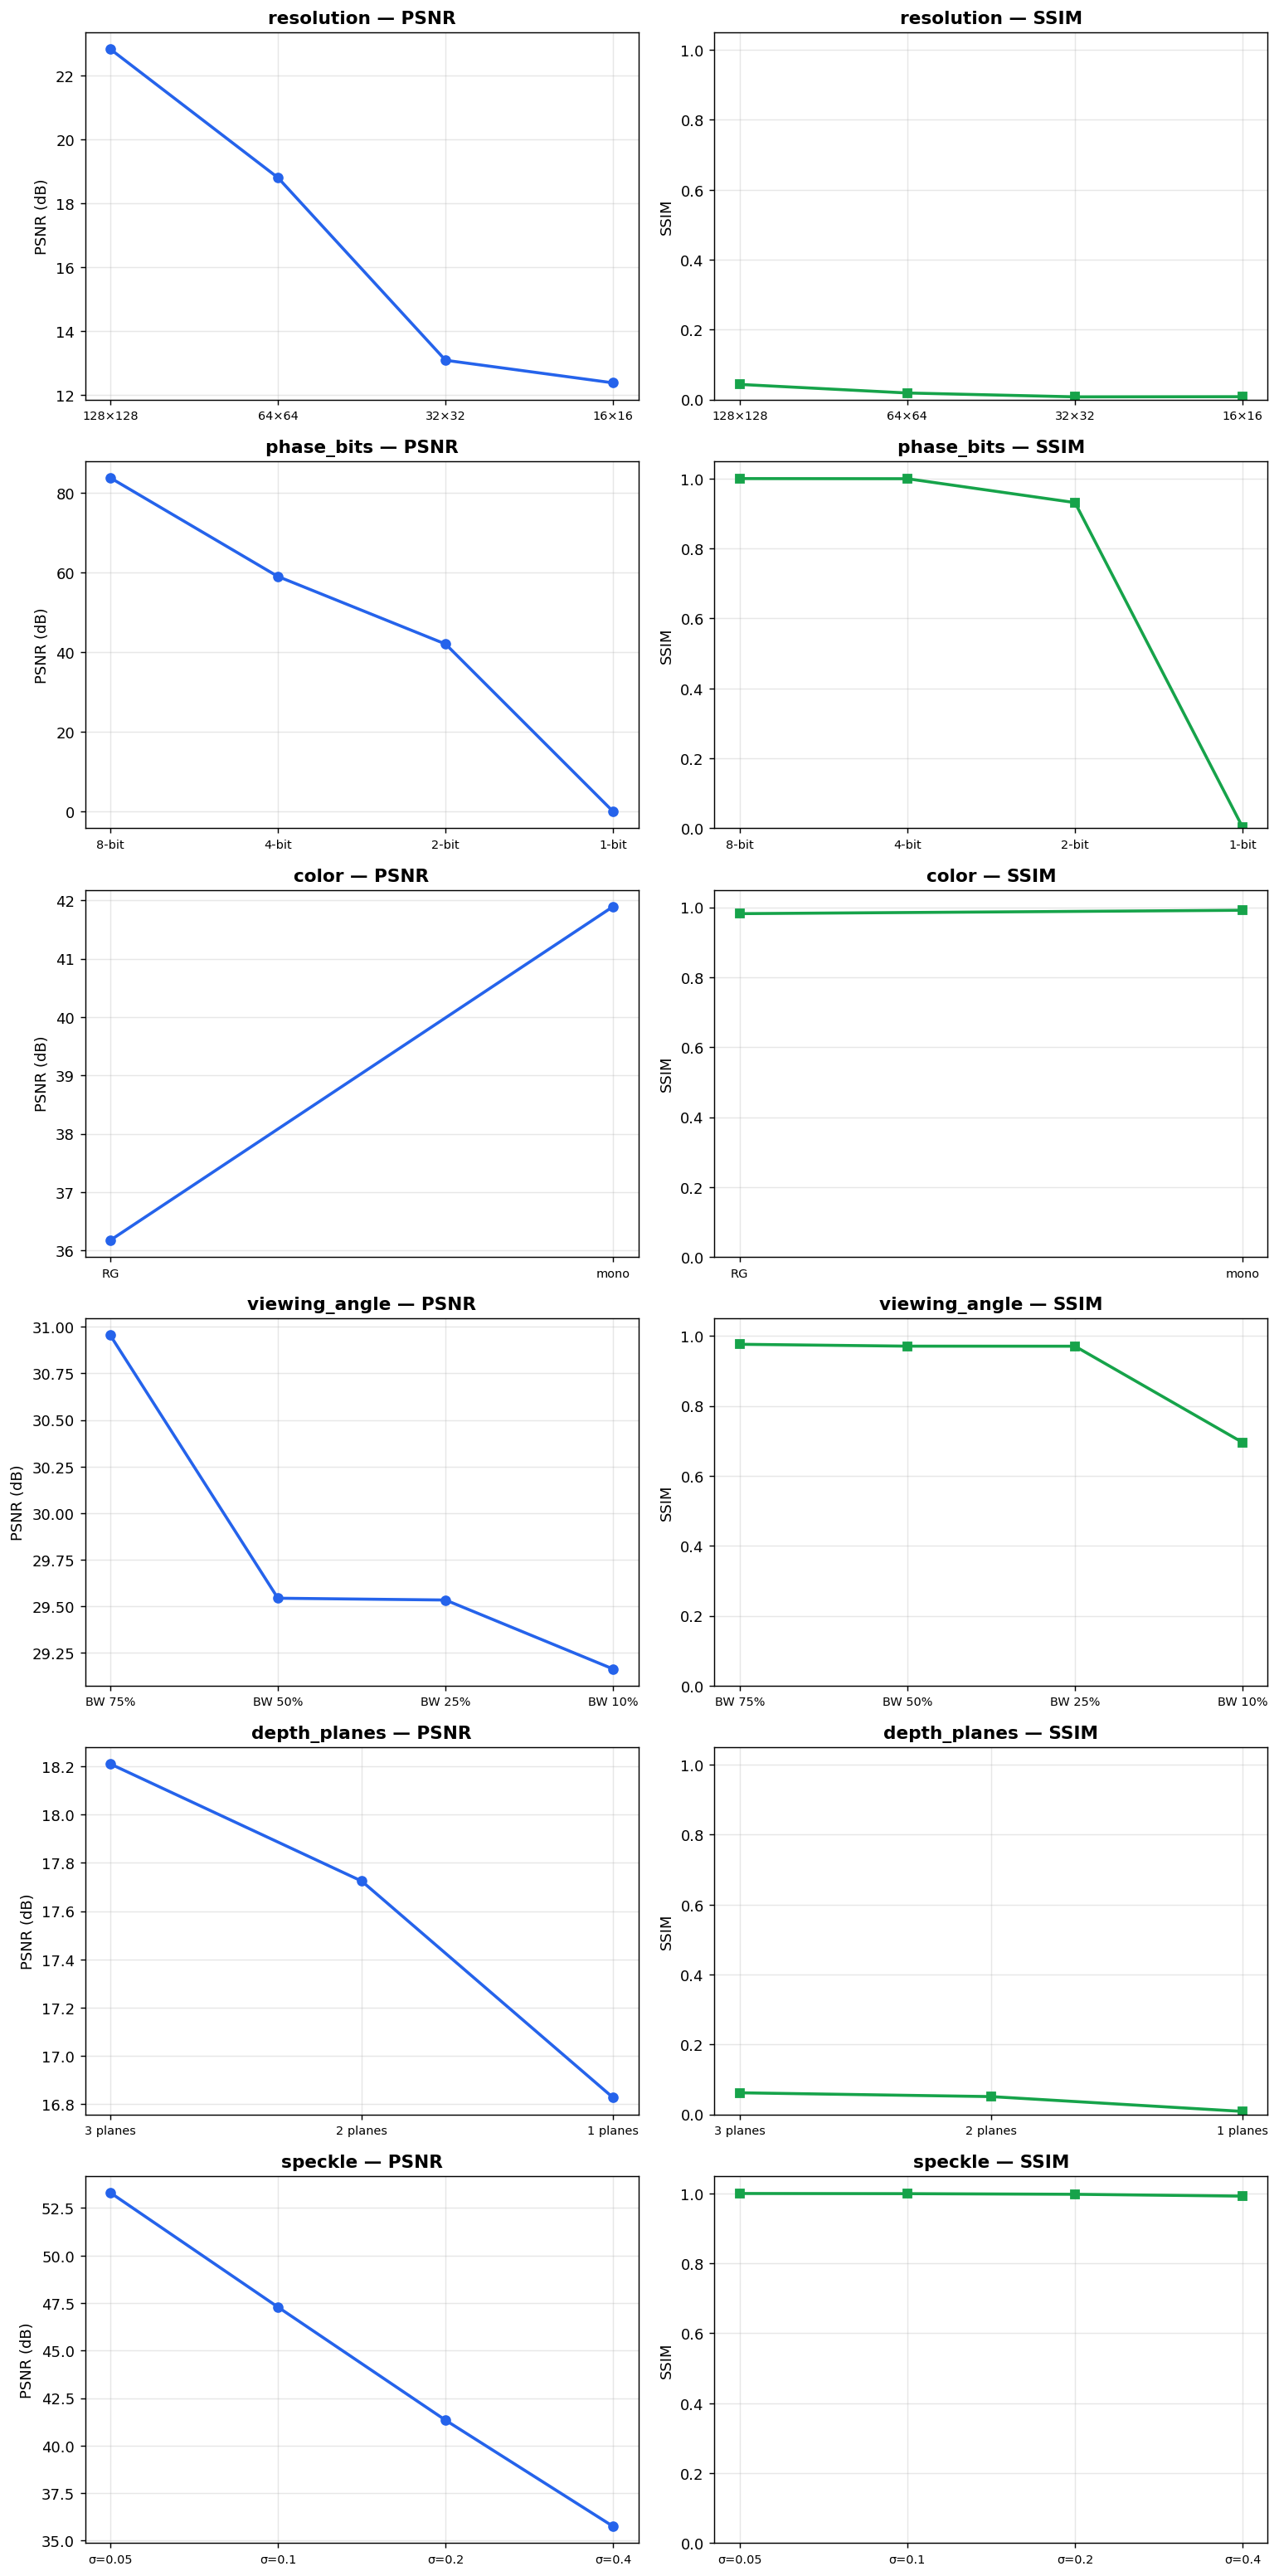
\includegraphics[width=\columnwidth]{metrics_summary_plot.png}
  \caption{PSNR and SSIM across the four reported degradation axes
  (resolution, phase quantisation, viewing angle, speckle). The metrics diverge
  most strongly under resolution loss, where PSNR remains a moderate
  $13$--$17\,\text{dB}$ while SSIM collapses below $0.05$.}
  \label{fig:metrics_summary}
\end{figure}
\begin{figure}[t]
  \centering
  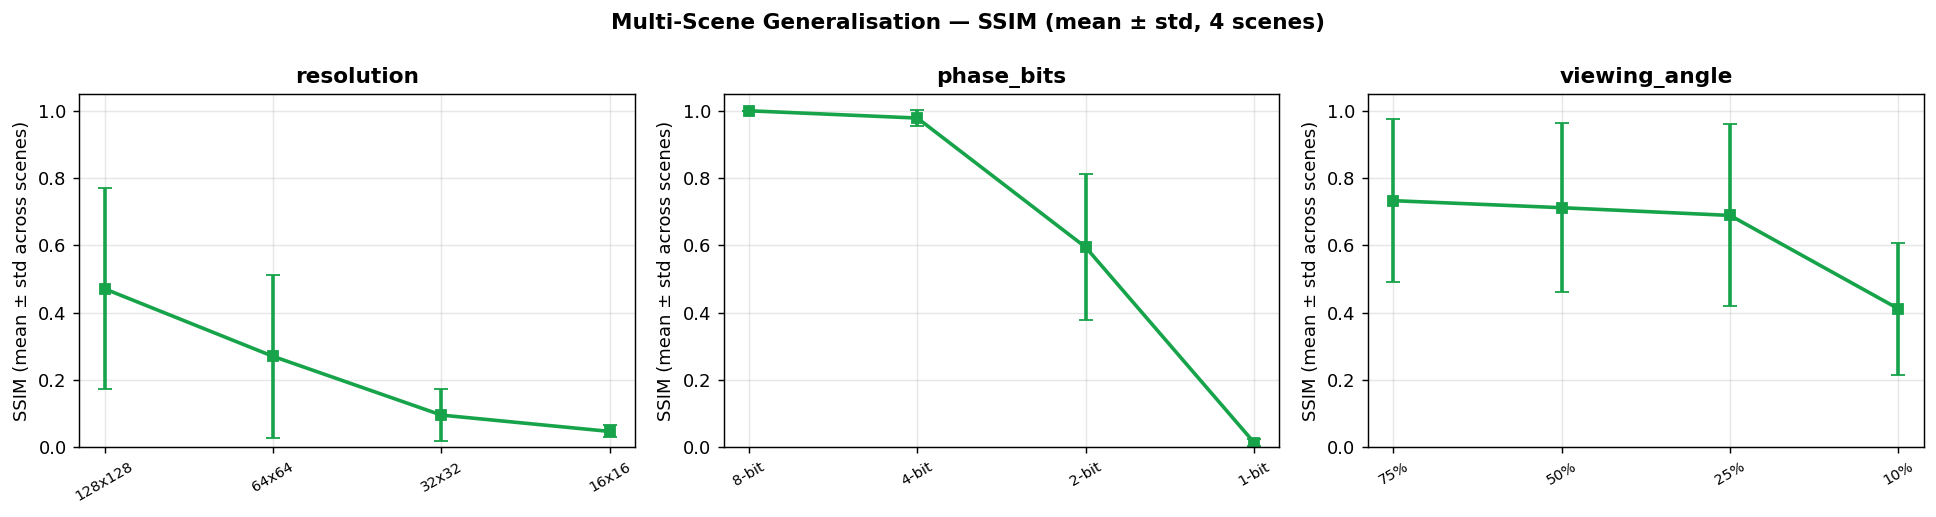
\includegraphics[width=\columnwidth]{multi_scene_summary.png}
  \caption{Multi-scene generalisation: SSIM (mean $\pm$ std across five scenes)
  for the resolution, phase-quantisation, and viewing-angle axes.}
  \label{fig:multiscene}
\end{figure}
\begin{table}[t]
  \centering
  \caption{Seed sensitivity (mean $\pm$ std across five GS seeds, reference scene)}
  \label{tab:seed}
  \begin{tabular}{llccc}
    \toprule
    Sweep & Param & PSNR (dB) & SSIM & LPIPS \\
    \midrule
    Phase & 8-bit & $82.93 \pm 0.70$ & $1.000 \pm 0.000$ & $0.000 \pm 0.000$ \\
    Phase & 4-bit & $59.23 \pm 0.22$ & $1.000 \pm 0.000$ & $0.000 \pm 0.000$ \\
    Phase & 2-bit & $45.66 \pm 0.79$ & $0.975 \pm 0.002$ & $0.019 \pm 0.004$ \\
    Phase & 1-bit & $35.93 \pm 0.22$ & $0.600 \pm 0.028$ & $0.202 \pm 0.011$ \\
    Res.  & 128   & $28.63 \pm 0.24$ & $0.860 \pm 0.009$ & $0.381 \pm 0.017$ \\
    Res.  & 64    & $25.55 \pm 0.59$ & $0.627 \pm 0.034$ & $0.583 \pm 0.022$ \\
    Res.  & 32    & $21.27 \pm 1.08$ & $0.239 \pm 0.031$ & $0.781 \pm 0.026$ \\
    Res.  & 16    & $17.23 \pm 1.09$ & $0.036 \pm 0.010$ & $0.895 \pm 0.021$ \\
    \bottomrule
  \end{tabular}
\end{table}
The PSNR/SSIM divergence is clearest in the resolution sweep
(Fig.~\ref{fig:metrics_summary}): at $16\times16$ effective resolution PSNR
remains a seemingly moderate $13$--$17\,\text{dB}$ while SSIM has collapsed below
$0.05$, so PSNR fails to register the structural destruction that SSIM and LPIPS
both capture. LPIPS additionally discriminates within the severe-degradation
regime where SSIM has saturated near zero (e.g.\ speckle $\sigma=1.0$ vs.\
$\sigma=\pi$). The multi-scene summary (Fig.~\ref{fig:multiscene},
Table~\ref{tab:multiscene}) shows the same ordering of axis severity holds across
content types, while seed sensitivity (Table~\ref{tab:seed}) confirms the
findings are not artefacts of a particular random initialisation: standard
deviations across seeds are small ($\le 1.2\,\text{dB}$ PSNR, $\le 0.034$ SSIM).
The large across-scene standard deviations in Table~\ref{tab:multiscene} are not
unstructured noise; Table~\ref{tab:perscene} breaks the phase-quantisation sweep
down per scene and shows the variance is driven by content frequency: the
smooth \textit{gaussian\_spots} scene retains $\text{SSIM}=0.655$ at 1 bit while
the broadband \textit{natural\_photo} falls to $0.089$, spanning almost the
entire range of the $0.273 \pm 0.198$ aggregate.

\begin{table}[t]
  \centering
  \caption{Across-scene summary (mean $\pm$ std, five scenes)}
  \label{tab:multiscene}
  \begin{tabular}{llcc}
    \toprule
    Axis & Param & SSIM & LPIPS \\
    \midrule
    Resolution    & 128 & $0.388 \pm 0.313$ & $0.659 \pm 0.220$ \\
    Resolution    & 16  & $0.052 \pm 0.020$ & $0.837 \pm 0.075$ \\
    Phase bits    & 2   & $0.636 \pm 0.250$ & $0.223 \pm 0.215$ \\
    Phase bits    & 1   & $0.273 \pm 0.198$ & $0.575 \pm 0.279$ \\
    Viewing angle & 25\% & $0.595 \pm 0.306$ & $0.435 \pm 0.257$ \\
    Viewing angle & 10\% & $0.362 \pm 0.202$ & $0.540 \pm 0.221$ \\
    \bottomrule
  \end{tabular}
\end{table}

\begin{table}[t]
  \centering
  \caption{Per-scene SSIM for the phase-quantisation sweep. The variance in
  Table~\ref{tab:multiscene} is content-driven: low-frequency scenes survive the
  1-bit transition far better than high-frequency ones.}
  \label{tab:perscene}
  \begin{tabular}{lcccc}
    \toprule
    Scene & 8-bit & 4-bit & 2-bit & 1-bit \\
    \midrule
    \textit{gaussian\_spots}   & $1.000$ & $1.000$ & $0.978$ & $0.655$ \\
    \textit{letters}           & $1.000$ & $0.997$ & $0.818$ & $0.241$ \\
    \textit{circle\_ring}      & $1.000$ & $0.978$ & $0.626$ & $0.213$ \\
    \textit{resolution\_chart} & $1.000$ & $0.947$ & $0.504$ & $0.165$ \\
    \textit{natural\_photo}    & $0.998$ & $0.749$ & $0.255$ & $0.089$ \\
    \bottomrule
  \end{tabular}
\end{table}

% ─── 6. Discussion ───────────────────────────────────────────────────────────
\section{Discussion}
\label{sec:discussion}

\subsection{The 1-bit Transition: an Unavoidable Twin Image}
A binary phase hologram with its two levels $\pi$ apart is, up to a global phase
factor, \emph{real-valued} (the phasors are $\pm j$, i.e.\ $j$ times a real
$\pm1$ pattern). Real-valued holograms---binary phase or binary amplitude
alike---are subject to the classical \emph{twin-image
problem}~\cite{gabor1948new}: because a real transmittance cannot encode the sign
of the diffracted field, the reconstruction necessarily contains the target
\emph{and} an equal-energy conjugate order. No Gerchberg--Saxton iteration can
remove the twin, since every member of the binary constraint set is real-valued.

This yields a concrete, falsifiable prediction: the fidelity penalty should
appear at exactly the bit depth at which the quantised hologram becomes
real-valued---$1$ bit---and should be \emph{structural} (a function of the
target's asymmetry) rather than stochastic. The data bear this out. The 1-bit
penalty is present for every scene and every seed, the reconstruction retains
coarse structure (SSIM $0.655$ on the reference scene, not a random field), and
the across-seed spread is tight ($\sigma_{\text{SSIM}} = 0.028$), exactly as
expected for a deterministic, symmetry-induced artefact. For $b \ge 2$ the
hologram is genuinely complex-valued, the real-valuedness constraint is lifted,
the twin image is no longer forced, and reconstruction is near-lossless.

The practical implication is sharpened accordingly: $2$ addressable phase bits
suffice for GS-style holography of these targets and $4$ bits are effectively
lossless; the distinctive cost of a $1$-bit device is the twin image, which is a
property of binary phase encoding itself rather than a failure of the retrieval
algorithm.

\subsection{Viewing-Angle Robustness}
The mildness of the viewing-angle axis is consistent with the spatial-frequency
content of the test scenes: the reference Gaussian spots are dominated by
low spatial frequencies, which survive aggressive circular bandwidth masking. The
larger across-scene variance and the steeper decline of \textit{resolution\_chart}
confirm that bandwidth tolerance is content-dependent---high-frequency detail and
wide fields of view are the first casualties of a reduced aperture. This suggests
that, for low-frequency or smoothly varying targets, designers may trade viewing
angle for other budget items with little perceptual penalty.

\subsection{Coherent Speckle as Pre-Reconstruction Phase Noise}
Modelling speckle as aperture-plane phase noise---rather than post-hoc
intensity noise---reproduces the correct coherent mechanism: small phase errors
interfere during propagation and only become visible in intensity beyond a
threshold ($\sigma \approx 0.6\,\text{rad}$ here). The soft knee in
Table~\ref{tab:speckle} gives an actionable tolerance for SLM phase accuracy and
optical-surface roughness.

\subsection{Metric Divergence}
No single scalar captures holographic quality. PSNR can remain moderate while
structure is destroyed---most visibly under resolution loss, where
$13$--$17\,\text{dB}$ coexists with $\text{SSIM} < 0.05$---so it must not be read
in isolation. SSIM tracks structural degradation but saturates near zero under
severe noise; LPIPS retains discrimination there (e.g.\ speckle $\sigma=1.0$
vs.\ $\sigma=\pi$). Reporting all three is therefore not redundant. Establishing which metric---or combination---best
predicts \emph{human} detection is the central question of Part~2.

\subsection{Limitations}
This study has several acknowledged limitations.
\textit{Single-wavelength simulation.} All experiments use $\lambda=532\,\text{nm}$;
multi-wavelength (RGB) holography introduces wavelength-dependent diffraction and
chromatic effects and is deferred to Part~2.
\textit{Limited scene diversity.} Four of the five scenes are synthetic and the
fifth is a single natural photograph; results on a broad corpus of natural or
photographic content---especially high-frequency, texture-rich imagery where GS
converges more slowly---remain to be characterised. The wide across-scene
variance we already observe (Tables~\ref{tab:resolution},~\ref{tab:viewing})
suggests content diversity is consequential and warrants a larger test set.
\textit{No human-observer validation.} The claim that simulation metrics predict
\emph{perceived} hologram quality is not yet validated with human subjects; Part~2
addresses this through a psychophysical forced-choice study.
\textit{Single retrieval algorithm.} Only classical GS is studied;
gradient-descent and learned holography~\cite{shi2021towards,
chakravarthula2019wirtinger} may exhibit different degradation-sensitivity
profiles.

% ─── 7. Conclusion ───────────────────────────────────────────────────────────
\section{Conclusion}
\label{sec:conclusion}
We presented \textsc{HoloForge}, a reproducible simulation framework for
systematic characterisation of degradation in phase-only holographic displays,
with all degradation operators applied in their physically correct domains.
Across four degradation axes, five scenes, and five random seeds we found phase
quantisation to be near-lossless down to 2 bits with a systematic, theoretically
predicted twin-image penalty at the 1-bit (binary) transition, near-lossless
behaviour of low-frequency content under aggressive viewing-angle reduction, a
quantified tolerance budget for coherent speckle, and a systematic divergence
between PSNR and perceptual metrics under resolution loss. These results establish a reproducible baseline and
motivate Part~2: a perceptual-threshold study mapping simulation metrics to human
detection thresholds, enabling hardware designers to make evidence-based SLM
specification trade-offs.

% ─── Reproducibility / Data Availability ─────────────────────────────────────
\section*{Code and Data Availability}
All source code, the experiment runner, the unit-test suite, and the raw result
CSVs and figures are available at
\url{https://github.com/ultramagnus23/HoloForge}. The complete result set is
regenerated by \texttt{python run\_experiments.py}.

% ─── References ──────────────────────────────────────────────────────────────
\bibliographystyle{IEEEtran}
\begin{thebibliography}{99}

\bibitem{maimone2017holographic}
A. Maimone, A. Georgiou, and J. S. Kollin, ``Holographic near-eye displays for
virtual and augmented reality,'' \textit{ACM Trans. Graph.}, vol.~36, no.~4,
pp.~1--16, 2017.

\bibitem{shi2021towards}
L. Shi, B. Li, C. Kim, P. Kellnhofer, and W. Matusik, ``Towards real-time
photorealistic 3D holography with deep neural networks,'' \textit{Nature},
vol.~591, pp.~234--239, 2021.

\bibitem{chakravarthula2019wirtinger}
P. Chakravarthula, Y. Peng, J. Kollin, H. Fuchs, and F. Heide, ``Wirtinger
holography for near-eye displays,'' \textit{ACM Trans. Graph.}, vol.~38, no.~6,
pp.~1--13, 2019.

\bibitem{peng2020neural}
Y. Peng, S. Choi, N. Padmanaban, and G. Wetzstein, ``Neural holography with
camera-in-the-loop training,'' \textit{ACM Trans. Graph.}, vol.~39, no.~6,
pp.~1--14, 2020.

\bibitem{choi2022time}
S. Choi, M. Gopakumar, Y. Peng, J. Kim, M. O'Toole, and G. Wetzstein,
``Time-multiplexed neural holography: a flexible framework for holographic
near-eye displays with fast heavily-quantized spatial light modulators,'' in
\textit{ACM SIGGRAPH 2022 Conf. Proc.}, 2022, pp.~1--9.

\bibitem{gerchberg1972practical}
R. W. Gerchberg and W. O. Saxton, ``A practical algorithm for the determination
of phase from image and diffraction plane pictures,'' \textit{Optik}, vol.~35,
pp.~237--246, 1972.

\bibitem{fienup1982phase}
J. R. Fienup, ``Phase retrieval algorithms: a comparison,'' \textit{Appl. Opt.},
vol.~21, no.~15, pp.~2758--2769, 1982.

\bibitem{gabor1948new}
D. Gabor, ``A new microscopic principle,'' \textit{Nature}, vol.~161,
pp.~777--778, 1948.

\bibitem{brown1966complex}
B. R. Brown and A. W. Lohmann, ``Complex spatial filtering with binary masks,''
\textit{Appl. Opt.}, vol.~5, no.~6, pp.~967--969, 1966.

\bibitem{lee1978computer}
W.-H. Lee, ``Computer-generated holograms: techniques and applications,''
\textit{Prog. Opt.}, vol.~16, pp.~119--232, 1978.

\bibitem{goodman2005introduction}
J. W. Goodman, \textit{Introduction to Fourier Optics}, 3rd ed. Englewood,
CO: Roberts and Company, 2005.

\bibitem{holoeye2023slm}
HOLOEYE Photonics AG, ``Spatial light modulators (LCoS phase),'' product
documentation, 2023. [Online]. Available: \url{https://holoeye.com/spatial-light-modulators/}

\bibitem{wang2004image}
Z. Wang, A. C. Bovik, H. R. Sheikh, and E. P. Simoncelli, ``Image quality
assessment: from error visibility to structural similarity,''
\textit{IEEE Trans. Image Process.}, vol.~13, no.~4, pp.~600--612, 2004.

\bibitem{zhang2018unreasonable}
R. Zhang, P. Isola, A. A. Efros, E. Shechtman, and O. Wang, ``The unreasonable
effectiveness of deep features as a perceptual metric,'' in
\textit{Proc. IEEE CVPR}, 2018, pp.~586--595.

\end{thebibliography}

\end{document}
